\documentclass[DIN, pagenumber=false, fontsize=11pt, parskip=half]{scrartcl}

\usepackage{amsmath}
\usepackage{amsfonts}
\usepackage{amssymb}
\usepackage{enumitem}
\usepackage[utf8]{inputenc} % this is needed for umlauts
\usepackage[ngerman]{babel} % this is needed for umlauts
\usepackage[T1]{fontenc} 
\usepackage{commath}
\usepackage{xcolor}
\usepackage{booktabs}
\usepackage{float}
\usepackage{tikz-timing}
\usepackage{tikz}
\usepackage{multirow}
\usepackage{colortbl}
\usepackage{xstring}
\usepackage{circuitikz}

\usetikzlibrary{calc,shapes.multipart,chains,arrows}

\title{Grundlagen der Rechnerarchitektur}
\author{Tim Luchterhand, Paul Nykiel (Abgabegruppe 117)}

\begin{document}
    \maketitle
    \section{Zähler}
    \begin{enumerate}[label=(\alph*)]
        \item $ $
            \begin{figure}[H]
                \centering
                \begin{tabular}{c|ccc|ccc}
                    \toprule
                    Flanke & $\text{state}_2[t]$ & $\text{state}_1[t]$ & $\text{state}_0[t]$ & $\text{state}_2[t+1]$ & $\text{state}_1[t+1]$ & $\text{state}_0[t+1]$ \\
                    \midrule
                    0 & 0 & 0 & 0 & 0 & 0 & 0\\
                    0 & 0 & 0 & 1 & 0 & 0 & 1\\
                    0 & 0 & 1 & 0 & 0 & 1 & 0\\
                    0 & 0 & 1 & 1 & 0 & 1 & 1\\
                    0 & 1 & 0 & 0 & 1 & 0 & 0\\
                    0 & 1 & 0 & 1 & 1 & 0 & 1\\
                    0 & 1 & 1 & 0 & 1 & 1 & 0\\
                    0 & 1 & 1 & 1 & 0 & 1 & 1\\
                    1 & 0 & 0 & 0 & 0 & 0 & 1\\
                    1 & 0 & 0 & 1 & 0 & 1 & 0\\
                    1 & 0 & 1 & 0 & 0 & 1 & 1\\
                    1 & 0 & 1 & 1 & 1 & 0 & 0\\
                    1 & 1 & 0 & 0 & 1 & 0 & 1\\
                    1 & 1 & 0 & 1 & 1 & 1 & 0\\
                    1 & 1 & 1 & 0 & 1 & 1 & 1\\
                    1 & 1 & 1 & 1 & 0 & 0 & 0\\
                    \bottomrule
                \end{tabular}
            \end{figure}
        \item
            \begin{eqnarray*}
                \text{state}_0[t+1] &=& \text{Flanke} \cdot (\overline{\text{state}_2[t]} \cdot \overline{\text{state}_1[t]} \cdot \overline{\text{state}_0[t]} + \\
                            && \overline{\text{state}_2[t]} \cdot \text{state}_1[t] \cdot \overline{\text{state}_0[t]} + \\
                            && \text{state}_2[t] \cdot \overline{\text{state}_1[t]} \cdot \overline{\text{state}_0[t]} + \\
                            && \text{state}_2[t] \cdot \text{state}_1[t] \cdot \overline{\text{state}_0[t]}) \\
                            && + \overline{\text{Flanke}} \cdot \text{state}_0[t]\\
                            &=& \text{Flanke} \cdot \overline{\text{state}_0[t]} +\overline{\text{Flanke}} \cdot \text{state}_0[t] \\
                            &=& \text{Flanke} \oplus \text{state}_0[t]
            \end{eqnarray*}
            \begin{eqnarray*}
                \text{state}_1[t+1] &=& \text{Flanke} \cdot (\overline{\text{state}_2[t]} \cdot \overline{\text{state}_1[t]} \cdot \text{state}_0[t] + \\
                            && \overline{\text{state}_2[t]} \cdot \text{state}_1[t] \cdot \overline{\text{state}_0[t]} +\\
                            && \text{state}_2[t] \cdot \overline{\text{state}_1[t]} \cdot \text{state}_0[t] +\\
                            && \text{state}_2[t] \cdot \text{state}_1[t] \cdot \overline{\text{state}_0[t]}) \\
                            && + \overline{\text{Flanke}} \cdot \text{state}_1[t] \\
                            &=& \text{Flanke} \cdot (\text{state}_1[t] \oplus \text{state}_0[t]) + \overline{\text{Flanke}} \cdot \text{state}_1[t]
            \end{eqnarray*}

            \begin{eqnarray*}
                \text{state}_2[t+1] &=& \text{Flanke} \cdot (\overline{\text{state}_2[t]} \cdot \text{state}_1[t] \cdot \text{state}_0[t] +\\
                            && \text{state}_2[t]  \cdot \overline{\text{state}_1[t]} \cdot \overline{\text{state}_0[t]} +\\
                            && \text{state}_2[t] \cdot \overline{\text{state}_1[t]} \cdot \text{state}_0[t] +\\
                            && \text{state}_2[t] \cdot \text{state}_1[t] \cdot \overline{\text{state}_0[t]}) \\
                            && + \overline{\text{Flanke}} \cdot \text{state}_2[t]\\
                            &=& \text{Flanke} \cdot (\overline{\text{state}_2[t]} \cdot \text{state}_1[t] \cdot \text{state}_0[t] +\\
                            &&\text{state}_2[t] \cdot \overline{\text{state}_1[t] \cdot \text{state}_0[t]}) +\\
                            &&\overline{\text{Flanke}} \cdot \text{state}_2[t]
            \end{eqnarray*}
        \item $ $
            \begin{figure}[H]
                \centering
                \begin{circuitikz}
                    \node[european xor port] at (2,1) (xor){};
                    \node at (0,0) (fl) {Flanke};
                    \node at (0,2) (s0) {$\text{state}_0[t]$};
                    \node at (4,1) (s0o) {$\text{state}_0[t+1]$};
                    \draw (fl) |- (xor.in 2);
                    \draw (s0) |- (xor.in 1);
                    \draw (xor.out) -| (2.5,1);
                \end{circuitikz}
            \end{figure}
            \begin{figure}[H]
                \centering
                \begin{circuitikz}
                    \node[european xor port] at (3,1) (xor){};
                    \node[european and port] at (6,2) (and1){};
                    \node[european not port] at (3,3) (not){};
                    \node[european and port] at (6,4) (and2){};
                    \node[european or port] at (9,3) (or){};
                    \node at(0,5) (fl) {Flanke};
                    \node at(0,0) (s0) {$\text{state}_0[t]$};
                    \node at(0,2) (s1) {$\text{state}_0[t]$};
                    \node at(11,3) () {$\text{state}_1[t+1]$};
                    \draw (fl) |- (not.in);
                    \draw (fl) |- (and2.in 1);
                    \draw (not.out) |- (and1.in 1);
                    \draw (xor.out) |- (and1.in 2);
                    \draw (s0) |- (xor.in 2);
                    \draw (s1) |- (xor.in 1);
                    \draw (s1) -| (and2.in 2);
                    \draw (and1.out) -| (or.in 2);
                    \draw (and2.out) -| (or.in 1);
                    \draw (or.out) |- (10,3);
                \end{circuitikz}
            \end{figure}
            \begin{figure}[H]
                \centering
                \begin{circuitikz}
                    \node[european not port] at (3,0)(not1){};
                    \node[european and port] at (3,2)(and1){};
                    \node[european nand port] at (3,4)(nand){};
                    \node[european and port] at (5,1)(and2){};
                    \node[european and port] at (5,5)(and3){};
                    \node[european or port] at(7,3)(or1){};
                    \node[european and port] at(12,3)(and4){};
                    \node[european not port] at(10,4.5)(not2){};
                    \node[european and port] at(12,5)(and5){};
                    \node[european or port] at(14,4)(and6){};
                    \node at(0,0) (s20) {$\text{state}_2[t]$};
                    \node at(0,1.7) (s10) {$\text{state}_1[t]$};
                    \node at(0,2.3) (s00) {$\text{state}_0[t]$};
                    \node at(0,3.7) (s11) {$\text{state}_0[t]$};
                    \node at(0,4.3) (s01) {$\text{state}_1[t]$};
                    \node at(0,6) (s21) {$\text{state}_2[t]$};
                    \node at(7.5,4) (fl) {Flanke};
                    \node at(15,4) (o) {$\text{state}_2[t]$};
                    \draw (1.2,6) -| (and3.in 1);
                    \draw (not1.out) -| (and2.in 2);
                    \draw (and1.out) -| (and2.in 1);
                    \draw (nand.out) -| (and3.in 2);
                    \draw (and2.out) -| (or1.in 2);
                    \draw (and3.out) -| (or1.in 1);
                    \draw (or1.out) |- (and4.in 2);
                    \draw (fl) |- (and4.in 1);
                    \draw (fl) |- (not2.in);
                    \draw (not2.out) -| (and5.in 2);
                    \draw (and4.out) -| (and6.in 2);
                    \draw (and5.out) -| (and6.in 1);
                    \draw (s21) -| (and5.in 1);
                \end{circuitikz}
            \end{figure}
    \end{enumerate}

    \section{Addierer und Subtrahierer}
    \begin{enumerate}[label=(\alph*)]
        \item $ $
            \begin{figure}[H]
                \centering
                \begin{tabular}{ccc|cc}
                    \toprule
                    $a$ & $b$ & $c_{-1}$ & $c$ & $s$\\
                    \midrule
                    0 & 0 & 0 & 0 & 0 \\ 
                    0 & 1 & 0 & 0 & 1 \\ 
                    1 & 0 & 0 & 0 & 1 \\ 
                    1 & 1 & 0 & 1 & 0 \\ 
                    0 & 0 & 1 & 0 & 1 \\ 
                    0 & 1 & 1 & 1 & 0 \\ 
                    1 & 0 & 1 & 1 & 0 \\ 
                    1 & 1 & 1 & 1 & 1 \\ 
                    \bottomrule
                \end{tabular}
            \end{figure}
            \begin{eqnarray*}
                c &=& a \cdot b \cdot \overline{c_{-1}} + \overline{a} \cdot b \cdot c_{-1} + a \cdot \overline{b} \cdot c_{-1} + a \cdot b \cdot c_{-1} \\
                &=& a \cdot b + c_{-1} \cdot (\overline{a} \cdot b + a \cdot \overline{b}) \\
                &=& a \cdot b + c_{-1} \cdot (a \oplus b) 
            \end{eqnarray*}

            \begin{eqnarray*}
                s &=& \overline{a} \cdot b \cdot \overline{c_{-1}} + a \cdot \overline{b} \cdot \overline{c_{-1}} + \overline{a} \cdot \overline{b} \cdot c_{-1} + a \cdot b \cdot c \\
                &=& \overline{a} \cdot (b \cdot \overline{c_{-1}} + \overline{b} \cdot c_{-1}) + a \cdot (\overline{b} \cdot \overline{c} + b \cdot c) \\
                &=& \overline{a} \cdot (b \oplus c_{-1}) + a \cdot \overline{(b \oplus c_{-1})} \\
                &=& a \oplus b \oplus c_{-1}
            \end{eqnarray*}

        \item $ $
            \begin{figure}[H]
                \centering
                \begin{circuitikz}
                    \node[european xor port] at (3,2) (xor){};
                    \node[european and port] at (5,0) (and1){};
                    \node[european and port] at (5,4) (and2){};
                    \node[european or port] at (7,2) (or){};
                    \node at(0,-1) (c) {$c_{-1}$};
                    \node at(0,2.5) (a0) {$a$};
                    \node at(0,1.5) (b0) {$b$};
                    \node at(2,4.5) (a1) {$a$};
                    \node at(2,3.5) (b1) {$b$};
                    \node at(8,2) () {$c$};
                    \draw (c) -| (and1.in 2);
                    \draw (a0) -| (xor.in 1);
                    \draw (b0) -| (xor.in 2);
                    \draw (a1) -| (and2.in 1);
                    \draw (b1) -| (and2.in 2);
                    \draw (xor.out) -| (and1.in 1);
                    \draw (and1.out) -| (or.in 2);
                    \draw (and2.out) -| (or.in 1);
                \end{circuitikz}
            \end{figure}
            \begin{figure}[H]
                \centering
                \begin{circuitikz}
                    \node[european xor port] at (3,1) (xor1){};
                    \node[european xor port] at (5,2) (xor2){};
                    \node at(0,0) (a) {$a$};
                    \node at(0,1.5) (b) {$b$};
                    \node at(0,3) (c) {$c_{-1}$};
                    \node at(6,2) (){$s$};
                    \draw (a) -| (xor1.in 2);
                    \draw (b) -| (xor1.in 1);
                    \draw (xor1.out) -| (xor2.in 2);
                    \draw (c) -| (xor2.in 1);
                \end{circuitikz}
            \end{figure}
        \item Schaltbild des 3-Bit-Addierers:
            \begin{figure}[H]
                \centering
                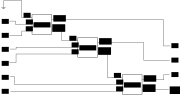
\includegraphics[width=\textwidth]{3BitAdder.eps}
            \end{figure}
        \item Schaltbild des 3-Bit-Addierers mit Subtraktionsfunktion. Die Schaltung aus der vorherigen Aufgabe wurde hier als Blockschaltbild verwendet:
            \begin{figure}[H]
                \centering
                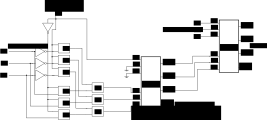
\includegraphics[width=\textwidth]{3BitKrassesDing.eps}
            \end{figure}
    \end{enumerate}
\end{document}
